\documentclass[10pt,a4paper]{scrartcl}
\pagestyle{empty}
\usepackage{a4} % alternativ \usepackage{a4wide}
\usepackage[utf8]{inputenc} % Unicode
\usepackage[ngerman]{babel} % Neudeutsche Silbentrennung (mehrsprachiges Dokument)
\usepackage{parskip} % Skip indentation of first row
\usepackage{graphicx} % Graphics support
\usepackage{longtable} % Tables across several pages
\usepackage{hyperref} % Hyperlinks
\usepackage[automark]{scrpage2} %kopf/fusszeile

\linespread{1.3}

\author{Danilo Bargen, Christian Fässler, Jonas Furrer} 
\title{Evaluation Datenbank\\Projekt BierIdee}

\pagestyle{scrheadings}
\ihead{SE2 Projekte} %linke Kopfzeile
\ohead{BierIdee} %rechte Kopfzeile

\begin{document}

\begin{titlepage}
	\maketitle
	\vspace{120mm}
	\thispagestyle{empty} % Don't start page numbers on this page
\end{titlepage}

\section{Evaluation}
\subsection{Vorwort}
Da es sich beim Projekt BierIdee - im Rahmen des Modules Software Engineering 2 Projekte - um ein Projekt mit stark beschränktem Zeitbudget handelt und zudem der Fokus auf der Anwendung des \textit{Rational Unified Process} liegt, wird diese Evaluation bewusst einfach gehalten. Die Produkt-Auswahl enthält auch subjektive Kriterien, da die Zeit für eine ausgwogene objektive Beurteilung fehlt.

\subsection{Einführung}
Es stellt sich die Frage wie sich unsere Problemdomain am besten modellieren lässt. Zwei Ansätze die sich herauskristalisiert haben sind Vektorräume und Graphen.


\subsection{Verfahren}. 
Zur Auswahl Stehen lediglich die Zwei Verfahren Vektorräume und Graphen. Diese Auswahl entstand einerseits durch eine Besprechung mit einem Mathematik-Dozenten und durch Eigenständige Modellierung.
\subsubsection{Vektorräume}
Bei der Modellierung mittels Vektorräumen werden die Bewertungen der Biere mittels Vektoren dargestellt. Jede Vektorkomponente stellt dabei ein Bier dar.
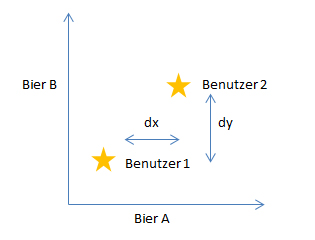
\includegraphics[scale=1]{vektor.jpg} 
Möchte man nun für einen Benutzer A eine Empfehlung erstellen, vergleicht man alle Bewertungen des gleichen Bieres der anderen Benutzer (selbe Vektorkomponente).
\subsubsection{Graphen}
\subsection{Auswahlverfahren}
Die Auswahl zwischen den beiden Produkten passiert anhand von Kriterien die einfach und schnell zu evaluieren sind. Dazu gehören:

\begin{description}
	\item[Laufzeit / Komplexität]
	\item[Produkte/Frameworks]Grober Überblick über vorhandene Frameworks, API's, DB Extensions welche bereits eine der angedachten Modellierungsvarianten ermöglichen.
	\item[Subjektivkriterien]Wie Empfehlungen durch dritte, oder Vorlieben von Teammitgliedern. (Auf diese Kriterien wird nicht mehr weiter eingegangen)
\end{description}

\subsection{Auswahl}
Bei den gewählten Kriterien ist ein direkter Vergleich nur schwierig möglich. Deshalb werden hier lediglich die Gedanke die zur Produktwahl geführt haben festgehalten.

\begin{description}
	\item[Popularität]Die Popularität von beiden Produkten ist hoch, für beide finden sich Zahlreiche Suchresultate sowie Hilfe durch die Community. Dieses Kriterium lässt keine eindeutige Gewichtung zu.
	\item[Features]Bei den Features bekommt Restlet mehr Gewicht. Die Features beider Frameworks sind weitgehen deckungsgleich. Restlet bietet allerdings noch Clientlibraries für Android. Da das Projekt BierIdee einen Android Client haben wird ist dies ein klarer Vorteil. Zudem bietet Restlet einen Built-in HTTP-Server welcher die Entwicklung voraussichtlich stark vereinfacht und beschleunigt.
	\item[Standards]Beide Produkte implementieren den \textit{JAX-RS} Standard.
\end{description}

\subsection{Evaluationsergebnis}
Das Auswahl der Kurzevaluation fiel auf Restlet. Den Ausschlag gaben die Gründe die im Punkt Auswahl unter Features nachzulsesen sind.

\end{document}